% source: 论文起草.md L1022-L1300

\section{光储可靠容量的计算}\label{apx:a}

{\sloppy\emergencystretch=3em
Goiri 等在 GreenSwitch 中按时段分配电网、光伏和电池功率，并追踪电池剩余电量\cite{q1ref04}（§5.2，原式（6）–（13））。本文沿用其功率与能量平衡，将目标改为求整个考察期均可供给的最大附加负荷 $L$。公共电网的持续供电已由式~\eqref{eq:q1-ptotal} 计入，附录仅核算自建电源增加的部分。\par}

将考察期划分为 $T$ 个长度为 $\Delta t$ 小时的时段。设备配置始终固定，$t$ 仅标记运行时段。设 $r_t$ 为可用光伏净功率（MW），由装机与同期气象条件转换得到~\cite{q1ref03}；$c_t,d_t$ 分别为充、放电功率（MW）；$e_t$ 为时段初的可动用电量（MWh）。每个时段须满足

\begin{equation}\label{eq:apxA-balance}
r_t+d_t\ge L+c_t,\qquad
e_{t+1}=e_t+\eta_c c_t\Delta t-\frac{d_t\Delta t}{\eta_d}.
\end{equation}

该式允许弃电。充电使用当时的供电余量，电池还需满足

\begin{equation}\label{eq:apxA-limits}
0\le c_t\le C_{\max},\quad 0\le d_t\le D_{\max},\quad
0\le e_t\le E_{\text{可用}},\quad e_{T+1}=e_1 .
\end{equation}

式~\eqref{eq:apxA-limits} 的电量上下限覆盖全部状态，包括期末。每个时段仅采用一种充放方向。周期首尾电量相同是本模型的边界条件，确保一个周期的供电可由该周期内的发电补回。于是

\begin{equation}\label{eq:apxA-f}
f_{\text{光储}}=\max\{L\ge0:\ \text{存在满足式~\eqref{eq:apxA-balance}、\eqref{eq:apxA-limits} 的全周期运行安排}\}.
\end{equation}

考察期决定结果的可外推范围。若仅校核一个晴天，所得上限只说明该昼夜循环能够维持。要估计场址在连续低日照期间的可保障容量，记录也应覆盖相应天气过程。若温度同时影响发电与机房冷却，可在式~\eqref{eq:apxA-balance} 左端加入固定的 $P_{\text{电网}}$，将右端的 $L$ 换成当时的设施负荷 $k_tP$，求所有时段均可维持的最大 IT 容量 $P$。

在给定总 IT 功率需求的条件下，分布式模型沿用集中式模型的设施用电核算方法，并将负荷分配至不同节点，同时计入跨节点通信所需的广域网功率。本文以 IT 功率作为算力需求的代理指标，设 D 为给定的总 IT 功率需求（MW），$D_{j,t}$ 为时段 t 分配至节点 j 的 IT 功率，其中包含服务器、存储和站内网络设备用电。各节点的分配应满足：

设 $k_{j,t}$ 为节点 j 在时段 t 的设施总功率与 IT 功率之比，用于计入冷却、配电等辅助用电；$P_{\text{广域网},t}$ 为归属于该计算任务的站外传输设备功率。全网实际所需功率为：

式中，站内网络设备已计入 IT 功率，并随节点 IT 负荷统一乘以设施用电倍率；站外广域网功率单独计入，不再乘以节点的设施用电倍率，以避免重复计算。分布式部署的供电灵活性体现为负荷可在满足节点供电额度、任务时延、带宽及所有者授权要求的地点之间分配，而不意味着总用电必然降低。上述结论以给定 IT 功率需求为前提，不直接等同于完成相同计算任务时的能耗比较。

\section{水电可持续供电功率的推导}\label{apx:b}

沿用《微型水电手册》附录 A-1 的水力功率推导\cite{q1ref06}。在流量 $Q$ 和净落差 $H$ 近似恒定的 $\Delta t$ 秒内，通过机组的水体体积为 $Q\Delta t$，质量为 $\rho Q\Delta t$，其中 $\rho$ 为水的密度。由重力势能关系，这部分水可提供的水力能量为

\begin{equation}\label{eq:apxB-energy}
\Delta E=\rho Q\Delta t\,gH.
\end{equation}

其中 $g$ 为重力加速度。若水力能转化为净电能的综合效率为 $\eta_{\text{水}}$，则将净电能除以时长，得到以瓦计的净电功率：

\begin{equation}\label{eq:apxB-power}
P_{\text{净}}=\frac{\eta_{\text{水}}\Delta E}{\Delta t}
=\eta_{\text{水}}\rho gQH.
\end{equation}

取淡水密度 $\rho\approx1000\ \mathrm{kg/m^3}$、$g\approx9.81\ \mathrm{m/s^2}$。由于 $1\ \mathrm{MW}=10^6\ \mathrm W$，将式~\eqref{eq:apxB-power} 换算为 MW 后，系数为 $1000\times9.81/10^6=0.00981$。最后取该净功率与机组装机容量 $X_{\text{水}}$ 中的较小值，即得正文式~\eqref{eq:q1-hydro}。

\section{有效用地与土地上限的估计}\label{apx:c}

\subsection{识别可建设的连续场址}\label{apx:c1}

将当地规划地块与地形、洪泛区和生态保护资料叠加，按事先声明的选址标准标出用途不符、地形不适宜或需要避让的区域~\cite{apxrefL01}。只在同一候选场址的边界内计算可用面积，重叠的排除区域合并后扣减一次。若剩余土地被道路、河道或保护区分隔，则分别检查各连续地块能否布置机房、配套设施和必要通道。即使面积充足，地块过窄或通行条件不足也可能使布局不可行。仅完成地图筛选时，所得容量应标明为基于面积的初筛上界。

若一个地区内有多个备选场址，可逐址重复以上步骤，分别记录 $A_{\mathrm{eff}}$ 和 $P_L(x)$。研究对象为单个集中式园区，各分散地块的容量不相加。只有在允许选择场址时，才在完成电、水、土地联合校核后比较各场址的可行容量。

\subsection{估计每增加 1 MW IT 所需的土地}\label{apx:c2}

同质化扩张方案更易于工程设计。mc生电区自古有“可堆叠”一说，即体现了这一设计哲学。

可用同一园区两期扩建资料估计 $a_{\mathrm{site}}$。令 $A_{\mathrm{IT},1}$ 和 $A_{\mathrm{IT},2}$ 为两期实际用于机房及其配套的地面面积，均已剔除发电用地和未动用的土地储备。若两期的共用固定设施基本相同，且同期额定 IT 容量从 $P_1$ 增至 $P_2$，则

\begin{equation}\label{eq:apxC-site}
a_{\mathrm{site}}\approx
\frac{A_{\mathrm{IT},2}-A_{\mathrm{IT},1}}{P_2-P_1},
\qquad P_2>P_1 .
\end{equation}

同样，若设计资料给出一个标准机房模块的新增占地与新增 IT MW，两者之比可直接作为边际用地强度。若只有某一期的资料，应先从机房侧用地中扣除可识别的 $A_0^{\mathrm{IT}}$，再除以额定 IT 容量。用地面积取地面占用范围；多层建筑应以总平面图核对建筑基底及室外配套。Epoch AI 可用于核对场址、建设阶段和 IT 功率，并追溯原始披露~\cite{apxrefL02}。项目面积仍须由同阶段的总平面图、规划文件或地块资料补齐。

线性近似要求扩建模块的机柜密度、建筑层数、冷却和配电布局大致稳定，新增地块也要能容纳相同布局。若跨越新建变电站、增设专用道路或改变建筑层数的设计节点，应分段估计固定用地和边际强度。若完整模块才可投运，式~\eqref{eq:q1-areq} 给出连续近似，实际容量应向下取到能够完整布置的模块数。在其他条件相同时，$a_{\mathrm{site}}$ 越大，土地可支撑的 IT 容量越低。缺少当地校准值时，可用有依据的区间展示这一影响。

\subsection{发电预留地与配套设施的边界}\label{apx:c3}

设 $A_{\mathrm{gen}}(x)$ 为自建电源及专属配套实际需要的园区内用地。对于给定预留方案，应满足

\begin{equation}\label{eq:apxC-gen}
A_{\mathrm{gen}}(x)\le A_e(x).
\end{equation}

式~\eqref{eq:apxC-gen} 检验发电配置能否建成，式~\eqref{eq:q1-areq} 按整块预留地扣减机房可用面积。若希望把未用完的预留地转给机房，可另设一个 $A_e$ 较小的候选方案。光伏场区内已含的升压站和道路只计一次；独立电池区有明确地块时计入实际需求。风电机位与道路的直接扰动面积、风机间距覆盖的整个项目面积应区分使用。采用哪种口径，取决于其余空间能否合法且实际用于机房建设~\cite{apxrefL03,apxrefL04,apxrefL05}。

园区外电源的土地另列为外部足迹，园区内为其服务的专属设施仍计入园区用地。按本研究水电方案的边界，水电设施自身占地不计入园区容量，采用该方案时应随结果说明。

给定发电预留面积后，火电按能完整布置的机组数计入供电。若分给某类机组的面积为 $A$，每台机组连同分摊后的专属配套需地 $a_{\mathrm{unit}}>0$，则最多容纳 $\lfloor A/a_{\mathrm{unit}}\rfloor$ 台。对风电和光伏，按分配到的合格面积乘以相应用地口径下的装机密度估算可建规模~\cite{apxrefL04,apxrefL05}。比较不同的 $A_e$ 时，每次用同一份用地分配重新计算电、水、土地三项上限，取三者中的最低值，再比较各方案的可持续容量。

\section{WUE特殊情况修正}\label{apx:d}

\section{水源数据缺失修补}\label{apx:e}

{\tolerance=2000\emergencystretch=1em
计算本地水压力通常需要河流基准流量 $Q_{\text{河流}}$、生态保留水量 $Q_{\text{生态}}$ 以及已有用户的净耗水量 $Q_{\text{其他耗水}}$。然而在实际工程中，上述数据（尤其是分散于生活、工业、农业各部门的 $Q_{\text{其他耗水}}$）常存在统计缺失。为此，当直接数据不足时，可通过以下三种途径先行获取水源可支持的新增取水量 $Q_{\text{可用}}$，再结合已知的 $Q_{\text{河流}}$ 与 $Q_{\text{生态}}$ 反推已有用户耗水量：\par}

\begin{equation}\label{eq:apxE-reverse}
Q_{\text{其他耗水}} = \max\left\{0,\; Q_{\text{河流}} - Q_{\text{生态}} - Q_{\text{可用}}\right\}
\end{equation}

\subsection{流域管理部门公开数据}\label{apx:e1}

优先检索取水河段对应的水文站实测流量、生态基流标准及分行业取用水统计数据，以补齐各项参数。若流域管理部门已直接发布对应断面与时段的\textbf{剩余可分配水量}或\textbf{可靠可供水量}，且该指标在核算时已扣除生态需水、现状取水及已批复的承诺额度，则可直接将其作为 $Q_{\text{可用}}$ 的取值依据。\cite{q1bref02,q1bref03,q1bref08,q1bref09}

\subsection{区域水资源分配模型}\label{apx:e2}

部分水资源管理较为成熟的地区建有区域水资源分配模型，能够将水权（即用户依法享有的取水权利，与 $Q_{\text{其他耗水}}$ 直接相关）、天然径流、回归水及水库调度纳入统一情景进行模拟。通过输入所在流域与拟建取水口位置等参数，即可输出该断面的\textbf{剩余可分配水量}，并将其作为 $Q_{\text{可用}}$。此类模型的典型代表包括美国得克萨斯州的 WAM/WRAP 模型、科罗拉多州的 StateMod 模型等。\cite{q1bref06,q1bref10}

\subsection{供水单位可交付水量}\label{apx:e3}

若数据中心并非直接从自然河道取水，而是接入市政或工业园区供水管网，则无需自行核算河道水压力，可改由供水单位针对该项目出具的\textbf{确认新增可交付水量}或正式\textbf{供水合同额度}作为项目侧的水量上限依据。

\section{实证场址的数据凭据、扩展复算与季节性背景}\label{apx:f}

\subsection{阿比林的四个规模数与宗地核查}\label{apx:f1}

同一个园区在不同边界下有四个不同的规模数，另有一个同边界下的整栋交付口径；混用会直接导致“高低”判断出错。表~\ref{tab:scales} 给出五者的边界与用途，第~\ref{sec:abilene}--\ref{sec:same-site}~节的比较全部按此表取值。

{\footnotesize
\begin{longtable}{@{}>{\raggedright\arraybackslash}p{0.13\textwidth}>{\raggedright\arraybackslash}p{0.36\textwidth}>{\raggedright\arraybackslash}p{0.15\textwidth}>{\raggedright\arraybackslash}p{0.25\textwidth}@{}}
\caption{阿比林园区的规模数、对应边界与用途。}\label{tab:scales}\\
\toprule
规模（MW IT） & 对应边界 & 数据来源 & 在正文中的用途 \\
\midrule
\endfirsthead
\toprule
规模（MW IT） & 对应边界 & 数据来源 & 在正文中的用途 \\
\midrule
\endhead
\bottomrule
\endlastfoot
$824.00$ & 2026 年拟建成的 8 栋单体建筑设备设计：$8\times(4\times25+3)$ & 总包逐项披露与开发商访谈 & 与同址、同阶段的资源上限直接对照 \\
$851.06$ & 上述 8 栋范围正常运行、全部使用网电时的资源上限（电、水、土地分别为 $851.06$、$1{,}266.15$、$962.75$） & 本模型计算 & 主校核结果，电力先触顶 \\
$895.60$ & 保留既有 8 栋不拆：在候选地上布 1 台 $100$ MW 干冷燃机（占 $10$ ha），余下 $13.36$ ha 用于扩建机房 & 本模型计算 & 业主不愿停运重建时的可行边界 \\
$980.75$ & 2033 年允许重排宗地并投运 $2\times100$ MW 干冷燃机的连续分配上限 & 本模型计算 & 回答“能否跨过 950 MW” \\
$927.00$ & 同上情景按每栋 $103$ MW IT 整栋投运，向下取整为 9 栋 & 本模型计算 & 交付口径的对照，第九栋布局尚未核实 \\
\end{longtable}
}

宗地核查的做法是：先按 Taylor 县宗地快照与城市规划区边界圈定运营宗地，得 $179.61$ ha（宗地外两座变电站 $5.85$ ha 在有效面积中单列、再作为固定用地 $A_0$ 扣回，两项相抵）；再用一期前两栋的租赁宗地 $38.43$ ha 与设计容量 $206$ MW IT 标定单位扩建用地强度 $a_s=0.18655$ ha/MW IT。

这里必须把两块地分清，否则 $962.75$ 与 $1{,}087.96$ 两个土地上限会互相矛盾。$179.61$ ha 是\textbf{已建成的运营宗地}（七宗，1、2 栋共宗），8 栋建筑本身占去其中大部分，只有允许重排之后才能整体用于 IT；真正的新增用地是四区块内、\textbf{宗地之外}的一块 $23.36$ ha 连续候选地（四区块内净余合计 $93.10$ ha，但分散在多个不相连的小块，最大连续单块即此 $23.36$ ha；若连同图示运维区一并计入，净余 $127.62$ ha、最大单块 $39.58$ ha）。这组数可以闭合检验：$179.61+93.10+48.37=321.08$ ha，与四区块 $330.19$ ha 相差 $9.11$ ha（道路与洪泛避让），其中 $48.37$ ha 是整带避让的规划缓冲——可见 $93.10$ ha 是\textbf{宗地之外}、四区块之内的净余，不是宗地内部的空地，两者不能相加两次，也不能互相替代。需要交代一处口径差：$179.61$ ha 是宗地面积（已含宗内道路与缓冲），$23.36$ ha 是扣除路网、站地、调蓄与规划缓冲后的净余，两者净毛口径不同，相加会略微高估可用地；因此 $1{,}087.96$ MW IT 只作为土地约束的\textbf{上界}使用，而由于电力先触顶，本节没有一个结论依赖它。两种边界对应两条扩建路径：\textbf{允许重排}时总土地盘为 $179.61+23.36=202.97$ ha，扣掉电源占地后全部可给 IT；\textbf{保留既有 8 栋}时只有这块候选地可用，扣掉一台燃机的 $10$ ha 后余 $13.36$ ha，正是 $895.60$ MW IT 的来源。之所以取 $23.36$ ha 而不取 $93.10$ ha，是因为机房必须落在连续地块上，分散的小块无法拼成机房。图~\ref{fig:candidates} 左半给出两种宗地口径下的剩余面积，右半给出保留 8 栋时扩建增量对用地强度的敏感性。

\begin{figure}[H]
\centering
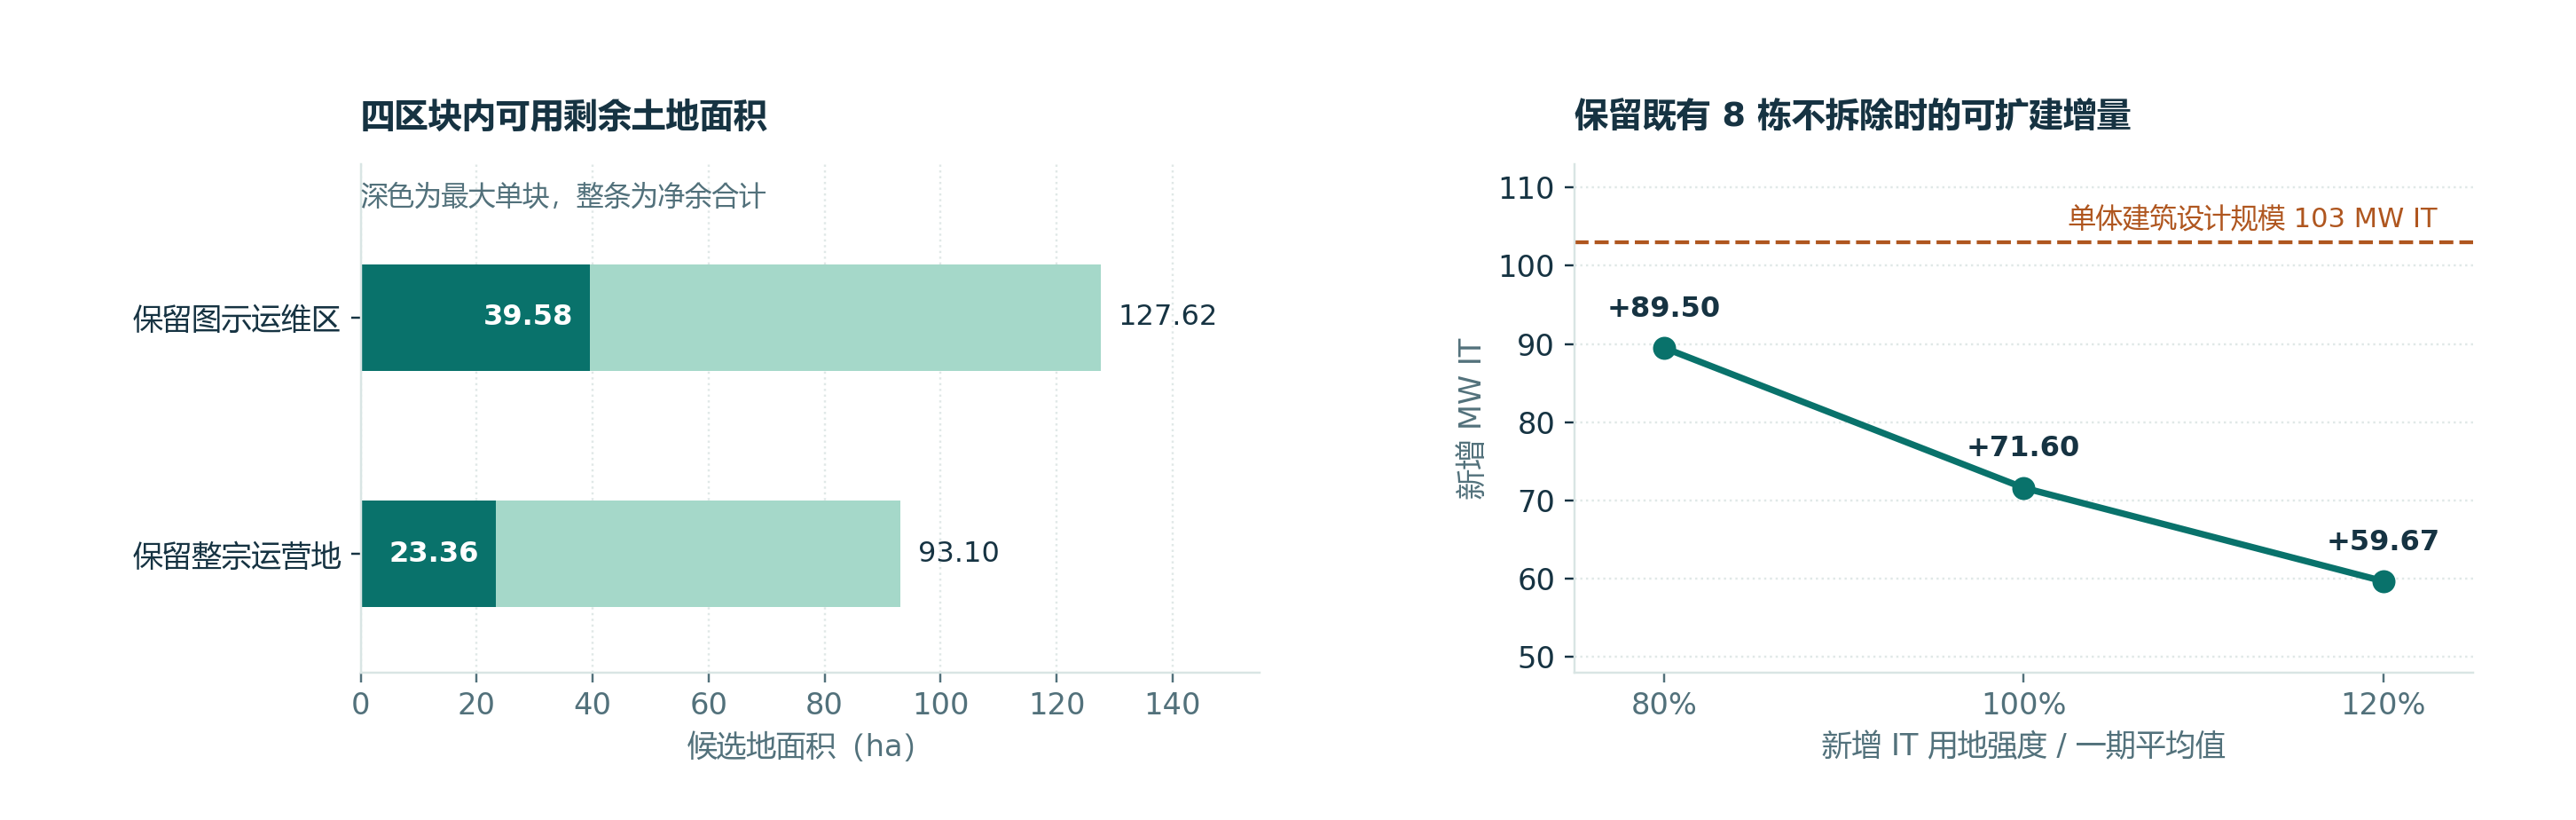
\includegraphics[width=0.76\textwidth]{figures/figF-1.png}
\caption{候选地剩余面积与“保留 8 栋”扩建增量。右图三点对应用地强度取一期平均值的 $80\%$、$100\%$、$120\%$，对应新增 $+89.50$、$+71.60$、$+59.67$ MW IT；按 $100\%$ 计即正文的 $895.60$ MW IT。}
\label{fig:candidates}
\end{figure}

\subsection{四地工程输入的取值与证据性质}\label{apx:f2}

表~\ref{tab:inputs} 逐项给出第~\ref{sec:migration}~节所用的四项输入及其证据性质。“披露”表示取自项目方公开文件，“运行统计”表示取自同址实测，“设计代理”表示用相邻口径的代用值，“同阶段标定”表示由该址自身的已建成规模反算，“情景假设”表示本研究设定的对照情景。读者可据此判断每个数能承受到什么程度的质疑。

{\footnotesize\setlength{\tabcolsep}{3pt}%
\begin{longtable}{@{}>{\raggedright\arraybackslash}p{0.135\textwidth}>{\raggedright\arraybackslash}p{0.08\textwidth}>{\raggedright\arraybackslash}p{0.065\textwidth}>{\raggedright\arraybackslash}p{0.075\textwidth}>{\raggedright\arraybackslash}p{0.085\textwidth}>{\raggedright\arraybackslash}p{0.065\textwidth}>{\raggedright\arraybackslash}p{0.065\textwidth}>{\raggedright\arraybackslash}p{0.08\textwidth}>{\raggedright\arraybackslash}p{0.125\textwidth}@{}}
\caption{四个场址的模型输入、取值与证据性质（2030 年基准）。}\label{tab:inputs}\\
\toprule
场址 & 电网功率（MW） & 满载倍率 $k$ & 可供水（m$^3$/h） & 取水强度（L/kWh IT） & 有效用地（ha） & 固定用地（ha） & 用地强度（ha/MW IT） & 证据性质 \\
\midrule
\endfirsthead
\toprule
场址 & 电网功率（MW） & 满载倍率 $k$ & 可供水（m$^3$/h） & 取水强度（L/kWh IT） & 有效用地（ha） & 固定用地（ha） & 用地强度（ha/MW IT） & 证据性质 \\
\midrule
\endhead
\bottomrule
\endlastfoot
冰岛凯夫拉维克 · Verne & $120$ & $1.20$ & $3.6$ & $0.02$ & $16$ & $0.15$ & $0.02$ & 运营披露 ＋ 情景假设 \\
新加坡丹戎吉岭 & $150$ & $1.19$ & $265.07$ & $2.4$ & $4.856$ & $0$ & $0.02594$ & 市场研究代理 ＋ 情景假设 \\
智利基利库拉 · Google & $65$ & $1.08$ & $180$ & $2.66$ & $15.9$ & $2.03$ & $0.1437$ & 需求预测 ＋ 环评水权 \\
澳大利亚悉尼西部 · SYD3 & $400$ & $1.15$ & $864$ & $1.2$ & $8.3$ & $0$ & $0.02594$ & 审批包络 ＋ 同阶段标定 \\
\end{longtable}
}

两处亚太场址共用同一份参数，是本研究为可比较性所作的处理，须在引用时保留：丹戎吉岭的用地强度直接转移自悉尼西部的整园平均值（$0.02594$ ha/MW IT），因为两地同为亚太高密度园区，而新加坡项目为 11 层建筑、实际密度尚未核实；凯夫拉维克的取水强度 $0.02$ L/kWh IT 取自闭式循环液冷的量级估计，运营商未公布同口径 WUE 数值。

\subsection{四地风光的季节性与弱光压力复算}\label{apx:f3}

第~\ref{sec:same-site}~节关于“小面积风光不足以支撑恒定负荷”的判断，依赖两点：一是各址风光资源本身存在季节性与年际差异，二是储能时长有限时连续低出力时段会直接决定可靠增量。四个场址 2016–2025 年的逐月统计见表~\ref{tab:seasons}，辐照与风速均取十年中位数，“月最低–最高”给出季节摆动的上下界。

{\footnotesize\setlength{\tabcolsep}{3pt}%
\begin{longtable}{@{}>{\raggedright\arraybackslash}p{0.135\textwidth}>{\raggedright\arraybackslash}p{0.125\textwidth}>{\raggedright\arraybackslash}p{0.095\textwidth}>{\raggedright\arraybackslash}p{0.075\textwidth}>{\raggedright\arraybackslash}p{0.095\textwidth}>{\raggedright\arraybackslash}p{0.145\textwidth}>{\raggedright\arraybackslash}p{0.145\textwidth}@{}}
\caption{四个场址的光照、风速季节性（2016–2025 年十年中位数）与光储可靠增量。}\label{tab:seasons}\\
\toprule
场址 & 年均日均辐照（kWh/m$^2$/日） & 辐照月最低–最高 & 年均风速（m/s） & 风速月最低–最高 & 光储可靠增量：全年／最低七天（MW IT） & 资源特征 \\
\midrule
\endfirsthead
\toprule
场址 & 年均日均辐照（kWh/m$^2$/日） & 辐照月最低–最高 & 年均风速（m/s） & 风速月最低–最高 & 光储可靠增量：全年／最低七天（MW IT） & 资源特征 \\
\midrule
\endhead
\bottomrule
\endlastfoot
冰岛凯夫拉维克 & $2.28$ & $0.05$–$5.01$ & $8.48$ & $6.34$–$10.22$ & $0.0022$／$0.0006$ & 冬月辐照近零（$100\times$ 摆动），平均风速四处最高 \\
新加坡丹戎吉岭 & $4.92$ & $4.31$–$5.68$ & $4.13$ & $2.93$–$5.58$ & $0.0175$／$0.0234$ & 辐照季节摆动最小（$1.3\times$），可用屋面极小 \\
智利基利库拉 & $5.93$ & $2.60$–$9.13$ & $1.88$ & $1.43$–$2.36$ & $0.0162$／$0.0131$ & 年均辐照四处最高，但夏冬差 $3.5\times$、风速最低 \\
澳大利亚悉尼西部 & $4.62$ & $2.44$–$6.65$ & $3.98$ & $3.62$–$4.53$ & $0.0382$／$0.0239$ & 辐照与风速均较平缓，风光本身不是限制因素 \\
\end{longtable}
}

\noindent 注：“光储可靠增量”指在固定电池配置下逐时调度可稳定多支撑的 IT 功率；“最低七天”取 2016–2025 年间光伏总出力最低的连续七天。两列均按附录~\ref{apx:f2} 的同一组参数计算。

表~\ref{tab:seasons} 说明三件事。第一，\textbf{资源的绝对量与可用量不是一回事}：基利库拉年均辐照最高（$5.93$ kWh/m$^2$/日）却受土地限制，丹戎吉岭季节摆动最小（$1.3\times$）却只有屋面可用，两地最终都拿不到与资源相称的增量。第二，\textbf{冰岛的“低辐照高风速”是唯一的互补结构}：冬季辐照近零而平均风速达 $8.48$ m/s，风电可以部分补上光伏的季节缺口，但该址的瓶颈始终在电网与水，不在风光。第三，\textbf{弱光窗口的影响是二阶的}：把电池配置固定，分别用 2025 年全年与十年最低七天求可靠增量，多数场址压到全年值的 $27\%$–$81\%$（凯夫拉维克最低，由 $0.0022$ 降到 $0.0006$），丹戎吉岭因水先触顶反而由 $0.0175$ 升至 $0.0234$（$+34\%$）；但所有数值都低于 $0.04$ MW IT，与各址联合容量相差两个数量级以上，瓶颈归属一个也没有改变。这说明“风光不可靠”不是某一年气象的偶然，而是 4 小时储能在恒定负荷要求下的结构性结果。

\subsection{敏感性与压力测试的复算网格}\label{apx:f4}

图~\ref{fig:sensitivity} 的两列基准（$851.06$ 与 $980.75$ MW IT）来自两条不同的分配路径：前者不设新增电源、只用网电，后者允许 $2\times100$ MW 干冷燃机投运并参与逐时调度。两条路径的敏感性不能互相代入，故分开列出。

{\footnotesize
\begin{longtable}{@{}>{\raggedright\arraybackslash}p{0.12\textwidth}>{\raggedright\arraybackslash}p{0.185\textwidth}>{\raggedright\arraybackslash}p{0.185\textwidth}>{\raggedright\arraybackslash}p{0.185\textwidth}>{\raggedright\arraybackslash}p{0.185\textwidth}@{}}
\caption{网电额度与供水额度的二维复算（单位：MW IT）。}\label{tab:grid}\\
\toprule
网电（MW） & 供水 $300$ m$^3$/h & 供水 $400$ m$^3$/h & 供水 $500$ m$^3$/h & 供水 $633.07$ m$^3$/h \\
\midrule
\endfirsthead
\toprule
网电（MW） & 供水 $300$ m$^3$/h & 供水 $400$ m$^3$/h & 供水 $500$ m$^3$/h & 供水 $633.07$ m$^3$/h \\
\midrule
\endhead
\bottomrule
\endlastfoot
$840$ & $595.74$／$599.78$ & $595.74$／$737.61$ & $595.74$／$737.61$ & $595.74$／$737.61$ \\
$960$ & $600.00$／$600.00$ & $680.85$／$793.64$ & $680.85$／$822.71$ & $680.85$／$822.71$ \\
$1{,}080$ & $600.00$／$600.00$ & $765.96$／$798.19$ & $765.96$／$907.82$ & $765.96$／$907.82$ \\
$1{,}200$ & $600.00$／$600.00$ & $800.00$／$800.00$ & $851.06$／$980.75$ & $851.06$／$980.75$ \\
\end{longtable}
}

\noindent 每格为“纯资源上限／允许 $2\times100$ MW 燃机时的最优容量”。

由表~\ref{tab:grid} 可以读出三点。第一，\textbf{纯资源口径下只有供水 $300$ m$^3$/h 的三格（网电 $960$、$1{,}080$、$1{,}200$ MW）与 $1{,}200$ MW 配 $400$ m$^3$/h 这一格由水先触顶}，其余全部由电先触顶；这说明“水比电更紧”只在低供水、高并网的角落成立。第二，\textbf{允许燃机后瓶颈是否转移取决于网电}：网电 $1{,}200$ MW 且供水不低于 $500$ m$^3$/h 时，瓶颈由电彻底转向土地，容量升到 $980.75$；网电降到 $1{,}080$ MW 或以下，燃机无法充分发挥，瓶颈仍落在电或水上。增量随供水额度单调上升：$1{,}200$ MW 配 $633.07$ m$^3$/h 时最大（$+129.69$ MW IT），供水降到 $400$ m$^3$/h 时增量归零（$800.00$／$800.00$），因为燃气与机房的取水已把额度用尽。第三，$840$\textbf{ MW 一栏的 $595.74\to599.78$ 说明燃机在强电约束下几乎无用}：电是硬上限，多一台机组只能补 $4$ MW 量级的调度缺口。

其余单因素复算如下：满载倍率 $k=1.3$ 时纯网电分支 $923.08$、重配分支 $1{,}000.03$；$k=1.4$ 时 $857.14$ 与 $980.75$。用地强度降至 $0.14924$ ha/MW IT 时重配分支升至 $992.92$。取水强度取 $0.2$ L/kWh IT 时两支均不受水约束（纯网电仍为 $851.06$，重配仍为 $980.75$）。候选地的规模还涉及一个口径选择：若\textbf{规定候选地只用于布置电源、剩余空地不并入机房}（保守口径），逐档放开 $0$／$10$／$20$／$23.36$ ha 时重配容量依次为 $851.06$／$921.99$／$962.75$／$962.75$ MW IT——$20$ ha 已足够容纳两台机组，再多的空地不再提升上限；若\textbf{允许剩余空地并入机房}（正文 4.3 采用的口径），$23.36$ ha 中扣掉两台机组的 $20$ ha 后还有 $3.36$ ha 可给 IT，容量才升到 $980.75$ MW IT。两种口径相差 $18.00$ MW IT，差别全部来自这 $3.36$ ha。需要强调的是，图 4-3 与表 F-4 的数值都是\textbf{资源上限}：若园区仍按 8 栋 $824$ MW IT 交付，$k$ 改善只增加资源余量而不改变交付规模——$k=1.2$ 时的 $1{,}000.00$ MW IT 并不意味着实际可多投运 $148.9$ MW IT。




